\documentclass[11pt,a4paper]{article}
\usepackage[utf8]{inputenc}
\usepackage[T1]{fontenc}
\usepackage{lmodern}
\usepackage[spanish,es-noquoting,es-tabla]{babel}
\usepackage[a4paper,margin=2.5cm]{geometry}
\usepackage{enumitem}
\usepackage{booktabs,array}
\usepackage{graphicx}
\usepackage{float}
\usepackage{multicol}
\usepackage[font=small,labelfont=bf,skip=3pt]{caption}
\usepackage[colorlinks=false,hidelinks]{hyperref}
\setlist{itemsep=1pt,topsep=2pt,parsep=0pt,leftmargin=1.2em}
\setlength{\parindent}{0pt}
\setlength{\parskip}{3pt}
\setlength{\emergencystretch}{3em}

\newcommand{\autor}{Máximo Sangiácomo}
\newcommand{\fuente}[1]{\par\vspace{1pt}{\footnotesize\raggedright #1\par}}
\newcommand{\nooficial}{Cálculo propio con datos públicos; no es una estimación oficial del BCRA.}

\title{\textbf{Anexos ilustrativos al proyecto de trabajo}\\[2pt]\large Gerente de Análisis Monetario (426 05)}
\author{\autor}
\date{}

\begin{document}
\maketitle
\vspace{-1.0cm}

\begin{center}\fbox{\parbox{0.96\linewidth}{\small
\textbf{Qué aprendí con datos públicos (tres mensajes).}
(1) \emph{Liquidez diaria (Eje~1)}: el calendario reduce 27--42\,\% el error de la circulación, pero no el de las cuentas corrientes de las entidades en el BCRA (98\,\% de la varianza diaria de la base): para ellas hacen falta factores programados y efectivo mínimo, información interna.
(2) \emph{Demanda de dinero (Eje~4)}: con el IPC oficial (2017--2026) no hay cointegración estable para el M2 ni para la base; el programa se apoya en la consistencia de fuentes y en reglas de seguimiento.
(3) \emph{Banda de tolerancia (Eje~4)}: funciona sin información futura, pero cubre 74--81\,\% de los desvíos, no el 90\,\% nominal: es el caso en que el indicador (vi) manda recalibrar.\\[2pt]
\textbf{Alcance.} Fuera del límite de cuatro páginas; el proyecto se entiende sin ellos. Resultados ilustrativos: \textbf{cálculos propios, no oficiales}. Código y pruebas automáticas, disponibles a pedido.}}\end{center}

\textbf{Datos.} Fuentes: BCRA, API de Estadísticas Monetarias v4.0 (descarga del 22-10-2026), e INDEC. La \emph{base} (serie 15) suma la \emph{circulación monetaria} (16) y las \emph{cuentas corrientes de las entidades en el BCRA} (15 $-$ 16); los \emph{billetes en poder del público} (17) son la circulación fuera de los bancos. El M2 109 es el M2 total; el 197, el transaccional privado (desde 2021, no alcanza para B y C). Tasas: plazo fijo (1189) y BAIBAR (11). INDEC: EMAE desestacionalizado e IPC nacional, éste sólo desde dic-2016 (se descarta un empalme previo de fuente no documentada). Los saltos grandes son hechos de política: el 10-07-2025 la base sube 30\,\% en un día, fecha en que, según el Informe Monetario Mensual de julio de 2025, el BCRA dejó de ofrecer las LEFI.

\section*{Anexo A. Anticipo del indicador (i): liquidez diaria (Eje 1)}
\textbf{Pregunta.} ¿Cuánto mejora el calendario el pronóstico a un día de la circulación y de las cuentas corrientes de las entidades en el BCRA frente al ingenuo (variación nula)? El indicador (i) se verifica con 60 observaciones en paralelo con datos \emph{internos}; esto es sólo un anticipo con datos públicos.
\textbf{Método.} $\Delta\ln X_t = \beta' c_t + \varepsilon_t$, con $c_t$: inicio y fin de mes, quincena, aguinaldo, diciembre y lunes; un ARIMAX agrega el rezago y el \emph{ensamble} promedia ambos. Reestimación cada 60 días hábiles sólo con el pasado; evaluación fuera de muestra desde ene-2022.

\begin{table}[H]\centering\small
\caption{Ensamble contra el ingenuo: MAE relativo ($p$ DM-HLN) y significancia económica.}
\setlength{\tabcolsep}{3pt}
\begin{tabular}{@{}lccccc@{}}
\toprule
Serie (ID) & ene-22 a oct-26 & desde 11-07-25 & últimos 60 días & Ahorro (pp & Cobertura\\
 & ($n=1166$) & ($n=310$) & ($n=60$) & de la base) & 90\,\%\\
\midrule
Circulación (16) & 0,58 ($<$0,001) & 0,65 ($<$0,001) & 0,73 (0,001) & 0,09 & 0,92\\
Billetes en público (17) & 0,73 ($<$0,001) & 0,86 (0,004) & 1,00 (0,49) & 0,06 & 0,95\\
Ctas.\ ctes.\ BCRA (15$-$16) & 1,00 (0,66) & 1,07 (0,99) & 1,09 (0,94) & $-$0,01 & 0,90\\
Base (15) & 1,00 (0,31) & 1,03 (0,87) & 1,04 (0,80) & 0,01 & 0,90\\
Base por componentes$^{a}$ & 0,99 ($<$0,001) & 0,99 (0,12) & 0,99 (0,21) & 0,02 & 0,91\\
\bottomrule
\end{tabular}
\fuente{Notas: MAE relativo: error absoluto medio del ensamble sobre el del ingenuo; $p$ unilateral. Ahorro: reducción del MAE diario en 2022--2026, en pp de la base (errores ponderados por el peso de la serie en la base); el MAE del ingenuo de la base es 1,65 pp. Cobertura: días dentro del intervalo del 90\,\%. $^{a}$ Circulación con el ensamble y cuentas corrientes con variación nula. Fuente: BCRA (último dato: 20-10-2026). \nooficial}
\end{table}

\textbf{Lectura.} En la circulación el ensamble reduce el error 27--42\,\%, con significancia aun en los últimos 60 días: esa parte del indicador (i) es alcanzable con datos públicos. En las cuentas corrientes, 98\,\% de la varianza diaria de la base, no mejora. Y la significancia estadística no basta: la base por componentes mejora con $p<0{,}001$, pero ahorra 0,02 pp por día, el 1\,\% del error, algo económicamente irrelevante. El total de factores de la base (serie 46) no sirve como predictor: por identidad, es la variación de la base del mismo día. \textbf{Conclusión}: la liquidez bancaria requiere los factores programados (Tesoro, divisas, vencimientos) y el período de cómputo del efectivo mínimo, información interna: el enfoque del Eje~1.

\section*{Anexo B. Demanda de dinero con el IPC oficial (Eje 4)}
\textbf{Pregunta.} ¿Hay una relación estable de largo plazo entre dinero real, actividad y costo de oportunidad que ancle el programa? \textbf{Alcance}: \emph{no} prueba la especificación del núcleo (inflación esperada, M2 privado): es un ejercicio con M2 total y base, IPC observado y tasas nominales, 2017--2026.
\textbf{Método.} Engle-Granger mensual: $\ln(M/P)_t = c + b_y \ln Y_t + b_i\, i_t + u_t$ ($Y$: EMAE) y modelo de corrección de errores (MCE), donde $g<0$ es la fracción del desvío corregida cada mes. Estabilidad: ventanas de 60 meses y CUSUM. Especificaciones fijadas de antemano; se informan todas.

\begin{table}[H]\centering\small
\caption{Demanda de dinero real con IPC oficial: coeficientes de largo plazo y diagnósticos.}
\setlength{\tabcolsep}{4.5pt}
\begin{tabular}{@{}lrrrrrr@{}}
\toprule
Dinero, tasa de plazo fijo & $b_y$ & $b_i$ & $p$ EG & $g$ ($t$) & $p$ CUSUM & Sin coint.\\
\midrule
M2 (2017--2026), principal & $-$0,82 & $-$0,23 & 0,82 & $-$0,05 ($-$2,1) & 0,14 & 100\,\%\\
Base (2017--2026) & $-$1,48 & $-$0,86 & 0,70 & $-$0,06 ($-$3,3) & 0,06 & 98\,\%\\
M2, antes de 2020 (2017--2019) & 0,59 & $-$0,92 & 0,86 & $-$0,33 ($-$3,1) & 0,60 & --\\
\bottomrule
\end{tabular}
\fuente{Notas: 116 meses (36 antes de 2020). $b_i$: semielasticidad. $p$ EG menor que 0,10 indica cointegración; $p$ CUSUM menor que 0,10 rechaza la estabilidad. “Sin coint.”: ventanas de 60 meses sin cointegración al 10\,\%. Con BAIBAR o tasa en logaritmos, $p$ EG de 0,88 a 0,93. Fuente: BCRA e INDEC; datos hasta ago-2026. \nooficial}
\end{table}

\textbf{Lectura.} \emph{No hay cointegración} en ninguna especificación ($p$ EG de 0,70 a 0,93) ni en casi ninguna ventana; la elasticidad ingreso negativa revela una relación inestable o mal especificada, que no se interpreta. Antes de 2020 los signos son los esperados, pero 36 meses no dan poder al test. \textbf{Conclusión}: no hay una demanda estable con estos datos; como prevé el núcleo, el programa se apoyaría en la consistencia de fuentes. Falta probar la especificación del núcleo: inflación esperada (REM), quiebres y M2 privado desestacionalizado.

\section*{Anexo C. Banda de tolerancia y desvíos del programa (Eje 4)}
\textbf{Pregunta.} Cuando el M2 o la base se desvían del programa, ¿el desvío es normal o requiere la nota del indicador (vi)?
\textbf{Método.} Cada mes desde ene-2021 se arma, con la información disponible, un programa a 1--3 meses y se guarda su error. Como en el núcleo, la banda sale de los percentiles del error fuera de muestra (5 y 95, sólo errores ya observados), calibrados para cubrir el 90\,\% nominal y revisados cada mes. Programas: (a) \emph{deriva} de 36 meses; (b) \emph{deriva estacional} (más el efecto típico de cada mes); (c) \emph{velocidad} constante; (d) \emph{demanda MCE} del Anexo~B con efectos mensuales, en ventanas de 48 meses; (e) MCE sin efectos mensuales. (c)--(e) usan IPC, EMAE y tasa observados: su error es un piso.

\begin{table}[H]\centering\small
\caption{M2 (109): error fuera de muestra y calibración de la banda; orígenes ene-2021 a may-2026.}
\setlength{\tabcolsep}{4pt}
\begin{tabular}{@{}lccccc@{}}
\toprule
Programa & MAE (\%) & MAE rel. & $p$ DM & $p$ DM vs. & Cobertura\\
($h=1$ / $h=3$ meses) & & a deriva & vs. deriva & estacional & 90\,\%\\
\midrule
(a) Deriva & 3,7 / 8,5 & 1,00 / 1,00 & -- & -- & 0,80 / 0,65\\
(b) Deriva estacional & 3,1 / 7,9 & 0,82 / 0,93 & 0,01 / 0,11 & -- & 0,72 / 0,58\\
(c) Velocidad & 3,3 / 6,0 & 0,88 / 0,70 & 0,14 / 0,04 & 0,70 / 0,13 & 0,91 / 0,94\\
(d) Demanda MCE & 3,2 / 6,7 & 0,86 / 0,78 & 0,14 / 0,12 & 0,63 / 0,24 & 0,74 / 0,80\\
(e) MCE sin ef.\ mensuales & 3,5 / 8,5 & 0,96 / 1,00 & 0,35 / 0,50 & 0,85 / 0,61 & 0,77 / 0,83\\
\bottomrule
\end{tabular}
\fuente{Notas: 65 orígenes comunes. $p$ DM: Diebold-Mariano-HLN unilateral. Cobertura: meses dentro de la banda armada con errores anteriores (41--43 meses en (d) y (e), que necesitan 24 errores previos). Ancho de la banda del 90\,\% a $h=3$: 21 pp en (a), 26 en (d), 31 en (c). En la base (15), (d) no supera a la deriva ($p\geq 0{,}14$) y cubre 0,68--0,81. Fuente: BCRA e INDEC; datos hasta ago-2026. \nooficial}
\end{table}

\textbf{Lectura.} (1) La demanda (d) no supera a la deriva estacional ($p\geq 0{,}24$) ni, al 10\,\%, a la deriva a 1 y 3 meses: no aporta más que la estacionalidad, coherente con el Anexo~B. (2) La velocidad mejora a la deriva a 2 y 3 meses porque conoce la inflación efectiva en plena desinflación, y cubre el 90\,\% sólo con una banda muy ancha. (3) Las bandas de (a), (b) y (d) cubren 58--81\,\%: según el indicador (vi), \emph{se recalibran} (más anchas o con más peso de los errores recientes) hasta acercarse al 90\,\%. (4) En jul-2025 a jun-2026, (d) deja fuera de banda un mes (ene-2026, figura~1), que llevaría su nota en diez días hábiles; la deriva, 7 de 12. En el BCRA, la banda usaría el error del programa vigente, incluido su escenario macro.

\begin{figure}[H]\centering
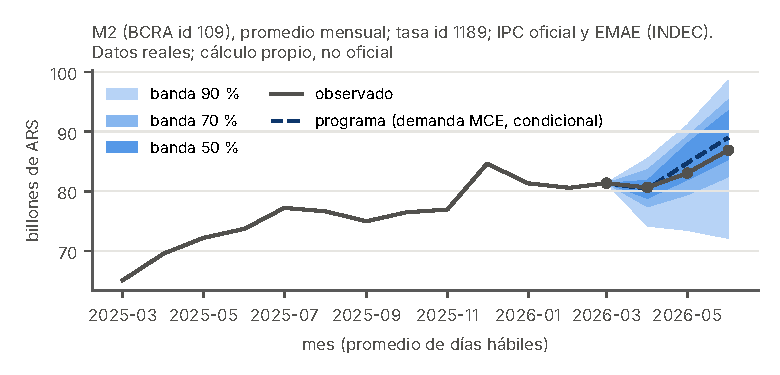
\includegraphics[width=0.66\linewidth]{codigo/salidas/fan_chart_real.pdf}
\caption{M2 (109), billones de \$, promedio mensual: observado, programa MCE armado en mar-2026 (condicional al IPC y al EMAE observados) y bandas del 50, 70 y 90\,\%. Fuente: BCRA e INDEC. \nooficial}
\end{figure}

\section*{Glosario}
\begin{multicols}{2}\footnotesize\raggedright
\begin{description}[leftmargin=0pt,itemsep=1pt,font=\normalfont\bfseries]
\item[Fuera de muestra.] Cada pronóstico usa sólo datos disponibles al hacerlo y se evalúa con datos que el modelo no vio (sin \emph{look-ahead}).
\item[Benchmark.] Referencia sin modelo: variación nula (A), deriva o deriva estacional (C). Un modelo útil debe superarla.
\item[MAE relativo.] Error absoluto medio del modelo sobre el del benchmark; 0,75 equivale a 25\,\% menos error.
\item[Diebold-Mariano (HLN).] Test de igual precisión de dos pronósticos, corregido para muestras chicas; con $p<0{,}10$ el modelo es más preciso.
\item[Cobertura.] Proporción de datos dentro del intervalo o la banda; con un 90\,\% nominal debería rondar 0,90.
\item[Cointegración y MCE.] Variables con tendencia que guardan una relación de largo plazo; el modelo de corrección de errores corrige cada mes una fracción del desvío.
\end{description}
\end{multicols}

\textbf{Límites.} En el BCRA se usarían datos internos en el entorno resguardado; EMAE e IPC se usan en su versión actual, no en tiempo real; A pronostica sólo a un día.
\end{document}
